%-------------------------------------------------------------------------------
% Cross-Signal Anomaly Detection for Enterprise AI-Agent Governance
% Draft paper #4 — fully synthetic evaluation; see README disclosure.
% Compile with: tectonic main.tex   (or pdflatex + bibtex)
%-------------------------------------------------------------------------------
\documentclass[10pt]{article}

\usepackage[margin=1in]{geometry}
\usepackage{times}
\usepackage{graphicx}
\usepackage{booktabs}
\usepackage{amsmath,amssymb}
\usepackage{multirow}
\usepackage{xcolor}
\usepackage[hidelinks]{hyperref}
\usepackage{microtype}

\newcommand{\code}[1]{\texttt{#1}}
\graphicspath{{../figures/}}

\title{Cross-Signal Anomaly Detection for Enterprise AI-Agent Governance:\\
A Taxonomy of Agent Misbehavior Classes and a Synthetic-Telemetry\\
Evaluation Framework}
\author{Draft --- for review}
\date{}

\begin{document}
\maketitle

\begin{abstract}
Enterprise AI agents execute tasks autonomously and emit rich execution
telemetry: tool calls, latencies, token and cost accounting, permission
requests, escalations, retries, and outputs. Today's governance regimes are
mostly post-hoc: audits, logs, and after-the-fact review. This paper asks
whether such telemetry supports \emph{pre-violation} detection --- flagging
agent misbehavior before the violating action completes --- and builds the
machinery to answer that question reproducibly. We contribute (i) a
machine-readable telemetry event schema for agent governance; (ii) a taxonomy
of nine agent misbehavior classes (scope creep, privilege-escalation attempts,
runaway loops, data exfiltration, prompt-injection compromise, cost anomalies,
silent failure masking, approval-gate circumvention, and cross-agent
collusion), each defined behaviorally with observable signals, a
violation-completion point, and a parameterized injection for instantiation;
(iii) a seeded synthetic telemetry generator that emits $\sim$50k sessions
with logged ground truth; and (iv) a detection benchmark comparing four
detector families --- static rule thresholds (D1), per-agent statistical
baselining (D2), Isolation Forest on session feature vectors (D3), and a Markov
transition-likelihood sequence model (D4) --- on per-class ROC/PR,
false-positive cost per agent-day, and detection lead time. On the synthetic
benchmark at a headline budget of 0.1 false positives per agent-day, D2 gives
the best overall ranking quality (ROC-AUC 0.93) and detects 70\% of injected
anomalies with a median of 21~s of lead time before violation completion;
D1's interpretable rules capture 63\%; D3 captures 41\%; the sequence model
D4 ranks weakly overall but carries unique signal on behavioral discontinuity.
Coverage varies sharply by class: the benchmark honestly exhibits the designed
gaps --- aggregate detectors are essentially blind to mid-session
prompt-injection compromise (recall $\le$ 0.02), and cross-agent collusion
eludes session-scoped detectors by construction. No production validation is
claimed; all results come from synthetic telemetry with illustrative
parameters.
\end{abstract}

%===============================================================================
\section{Introduction}
\label{sec:intro}
%===============================================================================

Autonomous agents are moving from demos into enterprise workflows: they read
and write documents, query databases, call external APIs, and escalate to
humans when policy demands. With autonomy comes an execution surface that
traditional governance was not designed for. A conventional audit asks
\emph{after the fact} what an actor did and whether it was permitted; an agent,
however, can complete hundreds of micro-actions per hour, and the actions that
matter --- an out-of-scope write, an egress of sensitive records, a loop that
burns budget --- may complete in seconds. Post-hoc review of agent activity is
therefore doubly weak: it arrives after the harm, and its volume defeats manual
inspection.

A different posture is available. Agent runtimes already stream telemetry:
every tool invocation, every permission request and its outcome, every retry
and escalation, every token and dollar spent. If that stream is scored online,
governance can shift from audit to \emph{early warning}: flag a session whose
behavior departs from the agent's established norm while there is still time to
intervene, gate, or revoke. This paper studies that shift, with three
questions:
\begin{itemize}
  \item \textbf{Q1 (representation).} What telemetry schema faithfully captures
        agent behavior at a level that supports anomaly detection? (Section~\ref{sec:telemetry}.)
  \item \textbf{Q2 (taxonomy).} What classes of agent misbehavior are
        observable in that schema, and how does each class manifest? (Section~\ref{sec:taxonomy}.)
  \item \textbf{Q3 (detection).} How do four practical detector families rank
        and cover these classes, what do they cost in false alarms per
        agent-day, and how much lead time do they buy before a violation
        completes? (Sections~\ref{sec:generator}--\ref{sec:sensitivity}.)
\end{itemize}

\noindent\textbf{Position within the literature.} LLM-agent safety research
predominantly evaluates task success and harm in interactive benchmarks
(AgentBench~\cite{agentbench}, ToolEmu~\cite{toolemu}, $\tau$-bench~\cite{taubench},
InjecAgent~\cite{injecagent}); insider-threat and host-intrusion detection
research has long studied behavioral anomaly scoring, including Markov chain
models of user behavior~\cite{yemarkov,yeung2003}; AIOps has industrialized
log-anomaly detection~\cite{he2021}; and drift detection formalizes how
baselines decay~\cite{gama2014}. What is missing is a bridge: a
\emph{governance-oriented} telemetry model and misbehavior taxonomy for
enterprise agents, evaluated online with a benchmark whose ground truth is
fully known. That bridge is this paper's contribution.

\noindent\textbf{Contributions.}
\begin{enumerate}
  \item A machine-readable \textbf{telemetry event schema} defining the
        governance-relevant event stream (Section~\ref{sec:telemetry}; artifact:
        \code{artifacts/telemetry\_event\_schema.json}).
  \item A \textbf{taxonomy of nine misbehavior classes}, each with a behavioral
        definition, observable signals, severity weight, an explicit
        \emph{violation-completion} point (the anchor for lead-time scoring),
        and a parameterized injection (Section~\ref{sec:taxonomy}; artifact:
        \code{artifacts/misbehavior\_taxonomy.json}).
  \item A \textbf{seeded synthetic generator} producing $\sim$50k sessions
        across 500 agents with injected anomalies and logged ground truth ---
        a reusable, byte-reproducible benchmark
        (Section~\ref{sec:generator}).
  \item A \textbf{detection benchmark} comparing four detector families on
        per-class ROC/PR, alert cost per agent-day, and detection lead time,
        including a deliberately reported \emph{coverage-gap matrix}
        (Sections~\ref{sec:detection}--\ref{sec:sensitivity}).
\end{enumerate}

\noindent\textbf{Scope and honesty statement.} The evaluation is entirely
synthetic. The generator encodes the anomaly classes it later asks detectors to
find, so measured performance is an upper bound on what the same detectors
would achieve on real telemetry. We deliberately keep some classes subtle ---
prompt-injection compromise is invisible to aggregate detectors by
construction, and cross-agent collusion is mostly out of reach of
session-scoped detection --- and report those gaps rather than tuning them
away (Section~\ref{sec:limitations}). No ServiceNow product internals,
customer data, or proprietary telemetry are described or used; all parameters
are illustrative, informed only by public literature.

%===============================================================================
\section{Related Work}
\label{sec:related}
%===============================================================================

\paragraph{LLM agent safety and security.}
Public frameworks name the risks: the NIST AI Risk Management
Framework~\cite{nistairmf} organizes govern/map/measure/manage functions
around scoped authority and human oversight, and the OWASP Top 10 for LLM
Applications~\cite{owasp} enumerates excessive agency, sensitive-information
disclosure, prompt injection, and unbounded consumption --- four classes our
taxonomy instantiates directly. Indirect prompt injection demonstrated that
agents can be steered by content they consume~\cite{greshake2023}, and
InjecAgent benchmarks the attack surface for tool-integrated
agents~\cite{injecagent}. MITRE ATLAS~\cite{atlas} catalogs adversary tactics
against AI systems, including exfiltration. Agent benchmarks such as
AgentBench~\cite{agentbench}, ToolEmu~\cite{toolemu}, and
$\tau$-bench~\cite{taubench} measure capability and harm in interactive
settings. Our work is complementary: rather than scoring harm in the loop, we
score the telemetry that any of these systems already emits, and we contribute
the governance-specific taxonomy that connects them.

\paragraph{Agent governance.}
Recent legal and policy work argues that agents require governance mechanisms
beyond model-level alignment: ex-ante constraints on the principal--agent
relationship, runtime oversight, and liability allocation~\cite{kolt2025}.
Multi-agent deployments additionally create systemic risks --- collusion,
coordination, and conflict --- that are properties of populations, not
individuals~\cite{multiagent2025}. Our cross-agent collusion class is a direct,
telemetry-observable instantiation of the latter concern, and our
lead-time framing is a quantitative version of the ex-ante/runtime contention.

\paragraph{Insider-threat and host-intrusion detection.}
The closest methodological ancestors are behavioral intrusion detection: early
work modeled user command sequences as Markov chains and flagged
low-likelihood transitions~\cite{yemarkov}, generalized to dynamic/static
behavioral models~\cite{yeung2003}. Insider-threat surveys~\cite{homoliak2019}
organize detection around deviations in access and activity patterns. These
methods operate on command or API streams quantitatively similar to our tool
call stream; the differences we introduce are the governance-oriented event
schema (permission requests, escalations, approval outcomes), the misbehavior
taxonomy, and the lead-time evaluation protocol against known
violation-completion points.

\paragraph{AIOps anomaly detection, outlier detection, and drift.}
Log-anomaly and anomaly-detection pipelines in AIOps are surveyed
extensively~\cite{he2021}; Isolation Forest~\cite{iforest} remains a standard
unsupervised baseline for multivariate point anomalies; drift
adaptation~\cite{gama2014} formalizes why static baselines decay. Our detector
set is deliberately conventional --- a rule baseline, robust per-agent
z-scoring, Isolation Forest, and a Markov sequence model --- because the
contribution is the evaluation framework and taxonomy, not a novel learner;
the framework is designed so stronger detectors can be dropped in behind the
same interface.

\paragraph{Precision/recall under class imbalance.}
For rare-class evaluation we report both ROC and precision--recall curves
following Davis and Goadrich~\cite{davis2006}, and we anchor operating points
to a budget in \emph{false positives per agent-day} rather than a bare
threshold, because in operations the alert rate is the binding constraint.

%===============================================================================
\section{Telemetry Model}
\label{sec:telemetry}
%===============================================================================

The telemetry model is the citable interface between an agent runtime (or
gateway) and any downstream detector. We define one event = one completed
action, with the following fields (artifact:
\code{artifacts/telemetry\_event\_schema.json}):

\begin{center}
\small
\begin{tabular}{@{}llp{7.4cm}@{}}
\toprule
Field & Type & Semantics \\
\midrule
\code{session\_id} & string & one task instance executed by one agent \\
\code{agent\_id} & string & static agent identifier \\
\code{ts} & float & completion time, epoch seconds; strictly increasing within a session \\
\code{event\_type} & enum & \{\code{tool\_call}, \code{permission\_request}, \code{escalation}, \code{retry}, \code{output}\} \\
\code{tool\_name} & string? & invoked tool (null for \code{output}) \\
\code{latency\_ms} & float & wall-clock duration of the action \\
\code{tokens} & int & tokens attributed to the event \\
\code{cost} & float & USD attributed to the event \\
\code{target\_scope} & string & \code{family:name} resource scope (e.g.\ \code{db:dev}) \\
\code{approved} & bool? & approval outcome for \code{permission\_request}/\code{escalation} \\
\bottomrule
\end{tabular}
\end{center}

Three modeling choices carry the governance semantics:
\begin{enumerate}
  \item \textbf{Permission events are first-class.} A denied
        \code{permission\_request} is evidence of an agent attempting to exceed
        its grants --- a governance signal with no analogue in classical log
        schemas. For a gated tool call, the detector can reconstruct whether an
        approval preceded it (a \emph{gate-consistent} call), followed it
        (\emph{post-hoc} approval), or never happened (\emph{approval gap}).
  \item \textbf{Scopes are declared and comparable.} Each agent declares a
        scope set; an event whose \code{target\_scope} lies outside it is an
        out-of-scope action by definition, and an ungated tool acting on a
        scope outside its tool family is a \emph{proxy bypass} candidate.
  \item \textbf{Retries and escalations are separated.} Retry counts measure
        silent failure absorption; escalations measure failure surfacing. Their
        ratio is a governance signal (silent failure masking).
\end{enumerate}

\noindent The subsequent detector suite is developed against this schema only.
Sessions with \code{output} terminate normally; a session is the unit of
scoring, with events scored online as a growing prefix
(Section~\ref{sec:detection}).

%===============================================================================
\section{Misbehavior Taxonomy}
\label{sec:taxonomy}
%===============================================================================

The taxonomy is the paper's core conceptual contribution: nine classes of
agent misbehavior that are \emph{observable in governance telemetry} and
stably defined across implementations. For detection lead time we additionally
require each class to define an unambiguous instant when the misbehavior
\emph{completes} --- without it, ``early warning'' has no referent. Severity
weights are illustrative ordinals (1--5), not calibrated risk figures.
Artifact: \code{artifacts/misbehavior\_taxonomy.json}.

\begin{center}
\small
\begin{tabular}{@{}p{2.5cm}p{6.2cm}p{4.9cm}c@{}}
\toprule
Class & Behavioral definition & Primary signals & Sev. \\
\midrule
Scope creep & agent acts on resources outside its declared task scope; out-of-scope fraction grows & out-of-scope ratio/count, novel scopes & 3 \\
Privilege-escalation attempts & repeated \emph{denied} permission requests accumulating within a session & denied count/ratio, new tools requested & 4 \\
Runaway loops & short tool cycle repeated far beyond necessity until budget boundary & pattern repetition, call count, cost vs baseline & 3 \\
Data exfiltration & read-heavy burst on sensitive scopes followed by external writes & egress count, egress token share, out-of-scope ratio & 5 \\
Prompt-injection compromise & mid-session behavioral discontinuity: foreign transition regime, aggregates unchanged & split-half log-likelihood drop, min-$k$ transition likelihood & 5 \\
Cost anomalies & token/spend drift vs task-class baseline with unchanged call structure & tokens/cost per call vs baseline & 2 \\
Silent failure masking & high retry counts, suppressed escalation, success-claiming output & retry ratio, zero escalations & 3 \\
Approval-gate circumvention & gated actions executed without prior approval: missing, post-hoc, or via proxy tools & approval gaps, post-hoc approvals, proxy bypasses & 4 \\
Cross-agent collusion & complementary halves of a violating pattern split across an agent pair in a short window & pairwise timing, shared novel scope, complementary roles & 5 \\
\bottomrule
\end{tabular}
\end{center}

\noindent\textbf{Violation completion anchors.} Table~\ref{tab:completion}
summarizes per class. These anchors drive the headline metric: detection lead
time = \code{violation\_ts} $-$ first detection timestamp. Positive lead time
means the detector fired while the violation was still avoidable.

\begin{table}[t]
\centering\small
\caption{Violation-completion anchors used for lead-time scoring.}
\label{tab:completion}
\begin{tabular}{@{}ll@{}}
\toprule
Class & Violation completes when \dots \\
\midrule
Scope creep & first out-of-scope action completes \\
Privilege-escalation attempts & 4th denied permission request completes \\
Runaway loops / cost anomalies & cumulative cost first exceeds $3\times$ agent baseline \\
Data exfiltration & last egress event completes \\
Prompt-injection compromise & final action of the hijacked pivot window completes \\
Silent failure masking & terminal output emitted while unescalated failures remain \\
Approval-gate circumvention & last circumventing action completes \\
Cross-agent collusion & second agent's final coordinated action completes (handoff occurred) \\
\bottomrule
\end{tabular}
\end{table}

Two design commitments distinguish the taxonomy from a list of attack types.
First, \emph{evidence lives in different signals for different classes}: scope
discipline for scope creep, denial dynamics for privilege escalation, timing
and volume for loops and cost drift, sequence structure for prompt injection.
A single detector cannot cover all nine, which is precisely why the benchmark
reports a class $\times$ detector matrix (Section~\ref{sec:detection}).
Second, \emph{the taxonomy names its own blind spots}: prompt-injection
compromise is defined by construction to leave aggregates unchanged, so we
predict near-total blindness for aggregate detectors and partial visibility for
sequence models; the benchmark then confirms it rather than hiding it.

%===============================================================================
\section{Synthetic Telemetry Generator}
\label{sec:generator}
%===============================================================================

Real governance telemetry with labeled misbehavior does not exist in public
form, and a benchmark for pre-violation detection requires \emph{known} ground
truth for when each violation completed. We therefore build a seeded synthetic
generator (\code{code/generate\_agents.py}, \code{code/generate\_telemetry.py})
whose parameters are illustrative but whose structure follows the taxonomy.
Synthetic-data methodology is standard~\cite{syntheticdata}; the novelty here
is the governance-aware injection layer.

\paragraph{Agent population.} 500 agents across six task classes
(\emph{doc drafting, data analysis, customer support, code maintenance,
compliance audit, IT operations}). Each agent receives: a task class with a
canonical workflow; a per-agent first-order Markov chain over its permitted
tools (the class template perturbed by a Dirichlet draw, masked to the agent's
permissions); declared scopes (\code{workspace:*, db:dev, sandbox:*, \dots});
a session rate (4--18 sessions/day); and an analytic cost baseline derived
from its own stationary distribution and the illustrative price table.

\paragraph{Benign sessions.} Session lengths follow a clipped negative binomial
(mean $\approx$7 tool calls); tool sequences are sampled from the agent's own
chain; latencies and token counts are lognormal per tool; permission dynamics
include approved requests, denials with escalation, rare cached approvals, and
a small benign retry rate. Benign sessions are therefore \emph{noisy on
purpose}: approximately 8\% of benign sessions carry retry-heavy patterns, and
12\% contain at least one denied request --- the false-positive pressure that
makes the operating-point comparison meaningful.

\paragraph{Anomaly injection.} Each of the nine classes is a parameterized
mutation of a benign session, logged to ground truth with its violation
timestamp and the parameters used. The injectors are written to materialize
the class they represent: e.g.\ exfiltration appends a read burst on sensitive
scopes plus external writes (token-inflated) and anchors the violation at the
last egress; prompt-injection compromise re-samples the pivot window from the
\emph{most KL-divergent} foreign task-class chain restricted to permitted,
non-egress tools, draws 12 candidate realizations and commits the one most
divergent under the agent's own chain, preserves all per-call latency/token/
cost draws, family-consistently re-scopes tools, and inserts gate-consistent
approvals where needed --- so that by construction no aggregate or policy rule
trips; runaway loops append a repeating cycle (length 1--3, repeated 10--24
times); silent-failure masking injects a retry storm and deletes escalation
events, then verifies the session has \emph{at least} the minimum retry count
of the injected pattern (injecting additional retries on insufficient
sessions) so the class always materializes as defined.

\paragraph{Corpus and reproducibility.} The principal corpus (seed 42) contains
\textbf{49{,}377 sessions} and \textbf{525{,}123 events} over 10 simulated days
($\approx$9.9 sessions/agent-day), with \textbf{985 injected anomalies}
(2.00\%; 108--111 per class). Sessions are split 60/40 into calibration
(29{,}622) and evaluation (19{,}755) sets; all injections land in the
evaluation split, the calibration split is verified anomaly-free, and
detectors are only ever fit on calibration data. Regeneration is
byte-reproducible: SHA-256 checksums of both generated CSVs are recorded in
\code{data/generation\_metadata.json} and verified by re-running the pipeline
(identical checksums).

%===============================================================================
\section{Detection Pipeline and Evaluation}
\label{sec:detection}
%===============================================================================

\paragraph{Feature extraction.} All detectors consume one shared feature vector
per session (\code{code/features.py}), computed to be well defined on any
prefix of a session just as on a complete one --- so a threshold calibrated on
complete sessions applies unchanged to online prefixes. The 38 features span
volume/cost, latency, permission behavior, retries/escalations, scope
discipline, gate discipline (approval gaps, post-hoc approvals, proxy
bypasses), repetition structure, and sequence likelihood under the agent's own
calibrated chain (mean step log-probability, min-3 step mean, split-half
drop).

\paragraph{The four detector families.}
\begin{itemize}
  \item \textbf{D1 --- static rule thresholds} (operational baseline): a
        weighted sum of normalized exceedances over interpretable rules
        (out-of-scope ratio, denied-request count, retry-ratio-with-no-escalation,
        egress token share, budget ratio, pattern repetition, gate bypasses).
  \item \textbf{D2 --- per-agent statistical baselining}: robust $z$-scores of
        each governance signal against the agent's own history (scale =
        $\max(\text{IQR-based},\ \text{per-signal floor})$), session score =
        max positive $z$. Agents with insufficient history fall back to
        task-class statistics; per-signal floors are required because several
        governance signals are zero-inflated (a robust scale collapses to zero).
  \item \textbf{D3 --- Isolation Forest}~\cite{iforest} on session feature
        vectors (log-transformed heavy-tailed features, standardized), trained
        on \emph{mixed-length prefix} rows so that the model is meaningful when
        applied to partial sessions.
  \item \textbf{D4 --- Markov transition-likelihood sequence model}:
        per-agent first-order chains over tool calls (Dirichlet-smoothed),
        score = max of two robust $z$-scored statistics --- min-3 step
        log-likelihood (foreign transition windows) and split-half drop
        (mid-session regime change).
\end{itemize}

\paragraph{Protocols.} Detectors are fit on 75\% of the calibration split;
operating thresholds are selected on the remaining 25\% (\emph{out-of-sample})
to match a target alert budget in false positives per agent-day; the
evaluation split is then scored by those same models, so the reported
operating points are in-sample nowhere. Lead time is measured by rescoring
each anomalous session on growing prefixes with the same feature function,
recording the first prefix timestamp at which the operating threshold is
crossed, and comparing it with the ground-truth violation timestamp.
Detection rate counts sessions crossing at any prefix (a slightly permissive
protocol than end-of-session classification and reported as such); ROC/PR is
computed end-of-session, one class versus benign, on the evaluation split.

\paragraph{Headline results.} Table~\ref{tab:overall} reports the overall
comparison at the headline budget (0.1 FP/agent-day).

\begin{table}[t]
\centering\small
\caption{Overall evaluation on the held-out split (985 anomalies / 18{,}770
benign sessions; all thresholds out-of-sample). FP/ad = realized false
positives per agent-day at the operating point.}
\label{tab:overall}
\begin{tabular}{@{}lcccccc@{}}
\toprule
 & ROC-AUC & PR-AUC & Recall & Precision & FP/ad & Lead time (pre-viol.\ rate / median) \\
\midrule
D1 static rules      & 0.890 & 0.686 & 0.625 & 0.738 & 0.115 & 0.48 / 21.9\,s \\
D2 per-agent baseline& \textbf{0.934} & \textbf{0.786} & \textbf{0.702} & \textbf{0.748} & 0.123 & \textbf{0.70 / 21.2\,s} \\
D3 isolation forest  & 0.900 & 0.547 & 0.410 & 0.676 & 0.102 & 0.31 / 11.2\,s \\
D4 Markov sequence   & 0.629 & 0.116 & 0.078 & 0.298 & 0.095 & 0.10 / 12.7\,s \\
\bottomrule
\end{tabular}
\end{table}

\noindent D2 leads overall: with per-agent baselining, 70\% of injections are
detected with a median of $\approx$21~s of lead time before the violation
completes, at an alert cost of 0.12 FP/agent-day. D1's static rules trail
modestly (63\% recall), confirming that hand-set policies retain real signal
once count gates and benign-noise floors are tuned honestly. D3's
unsupervised scoring generalizes worse at this alert budget, and D4 --- with
no aggregate features at all --- ranks near chance overall, exactly as a
sequence-only detector should on a corpus dominated by aggregate anomalies.

\paragraph{Per-class coverage.} Table~\ref{tab:coverage} is the paper's
coverage-gap matrix: recall per class at the headline budget, with ROC-AUC in
parentheses. Figure~\ref{fig:coverage} renders the same matrix as a heatmap.

\begin{table}[t]
\centering\small
\caption{Class $\times$ detector recall at 0.1 FP/agent-day (ROC-AUC in
parentheses). Bold: best per row.}
\label{tab:coverage}
\begin{tabular}{@{}lcccc@{}}
\toprule
Class & D1 & D2 & D3 & D4 \\
\midrule
Scope creep            & 0.48 (0.81) & \textbf{0.59 (0.95)} & 0.02 (0.82) & 0.04 (0.50) \\
Privilege escalations  & 0.55 (0.91) & \textbf{1.00 (0.98)} & 0.35 (0.96) & 0.02 (0.52) \\
Runaway loops          & 0.93 (0.98) & \textbf{1.00 (0.99)} & 0.72 (0.98) & 0.05 (0.65) \\
Data exfiltration      & \textbf{1.00 (0.999)} & \textbf{1.00 (0.99)} & \textbf{1.00 (0.998)} & 0.30 (0.84) \\
Prompt-injection comp. & 0.01 (0.47) & 0.01 (0.51) & 0.01 (0.49) & \textbf{0.02 (0.66)} \\
Cost anomalies         & 0.22 (0.94) & \textbf{1.00 (0.99)} & 0.86 (0.98) & 0.03 (0.52) \\
Silent failure masking & \textbf{0.85 (0.93)} & 0.43 (0.92) & 0.05 (0.83) & 0.00 (0.48) \\
Gate circumvention     & \textbf{0.87 (0.92)} & 0.56 (0.93) & 0.48 (0.97) & 0.18 (0.74) \\
Cross-agent collusion  & \textbf{0.73 (0.90)} & \textbf{0.73 (0.96)} & 0.23 (0.92) & 0.06 (0.71) \\
\bottomrule
\end{tabular}
\end{table}

\begin{figure}[t]
\centering
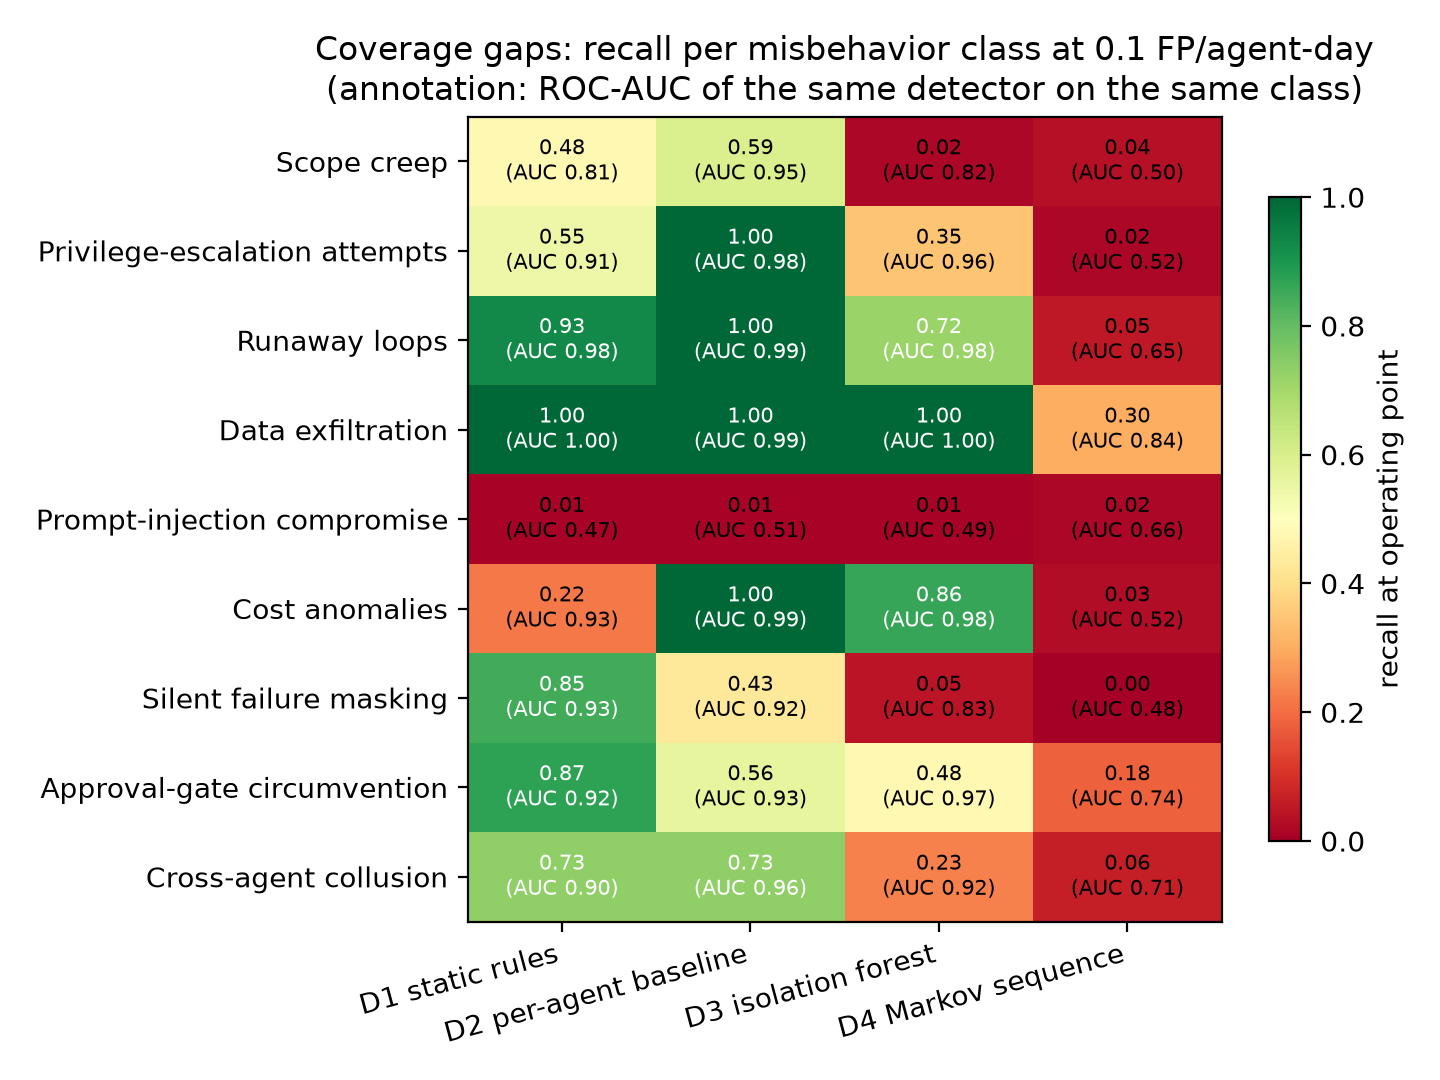
\includegraphics[width=0.86\textwidth]{fig1_coverage_gap_heatmap.png}
\caption{Coverage-gap heatmap: recall at 0.1 FP/agent-day with ROC-AUC
annotated. The two bottom-left cells are the designed gaps: aggregate
detectors are blind to prompt-injection compromise, and no session-scoped
detector fully covers cross-agent collusion.}
\label{fig:coverage}
\end{figure}

Four findings stand out:
\begin{enumerate}
  \item \textbf{Exfiltration is caught universally and early.} All of D1--D3
        reach recall 1.00 with AUCs $\ge$ 0.99, and every pre-violation
        detection lands $\approx$19~s before the data leaves the boundary ---
        the read burst is visible long before the egress completes.
  \item \textbf{Session-level detectors structurally miss cross-agent
        collusion.} The class is built so that each participating session is
        only mildly anomalous; D1/D2 still catch 73\% at the headline budget
        (via the shared out-of-scope destination) but at the cost of very
        long lead times, and D3 collapses to 0.23. Pair-level scoring is
        genuinely required; a session-scoped pipeline cannot fully solve this
        class.
  \item \textbf{Prompt-injection compromise is the designed blind spot.} D1--D3
        are at AUC $\approx$0.5 (chance) because by construction no aggregate
        or policy rule is tripped. D4 carries the only signal (AUC 0.66) ---
        the split-half drop and min-3 statistics see the regime change --- but
        even D4 converts only a sliver to recall at strict alert budgets.
        This gap is real and reported, not tuned away: behavioral-discontinuity
        detection at operational alert rates remains open.
  \item \textbf{Detector strengths are complementary, not redundant.}
        D1 owns silent-failure masking (0.85) and gate circumvention (0.87)
        where explicit policy structure dominates; D2 owns scope creep,
        privilege escalation, loops and cost drift where per-agent baselining
        dominates; D3's only clear edge is cost anomalies (0.86); D4 is the
        only detector with any prompt-injection signal. A production ensemble
        would combine these signal families rather than pick a winner.
\end{enumerate}

\begin{figure}[t]
\centering
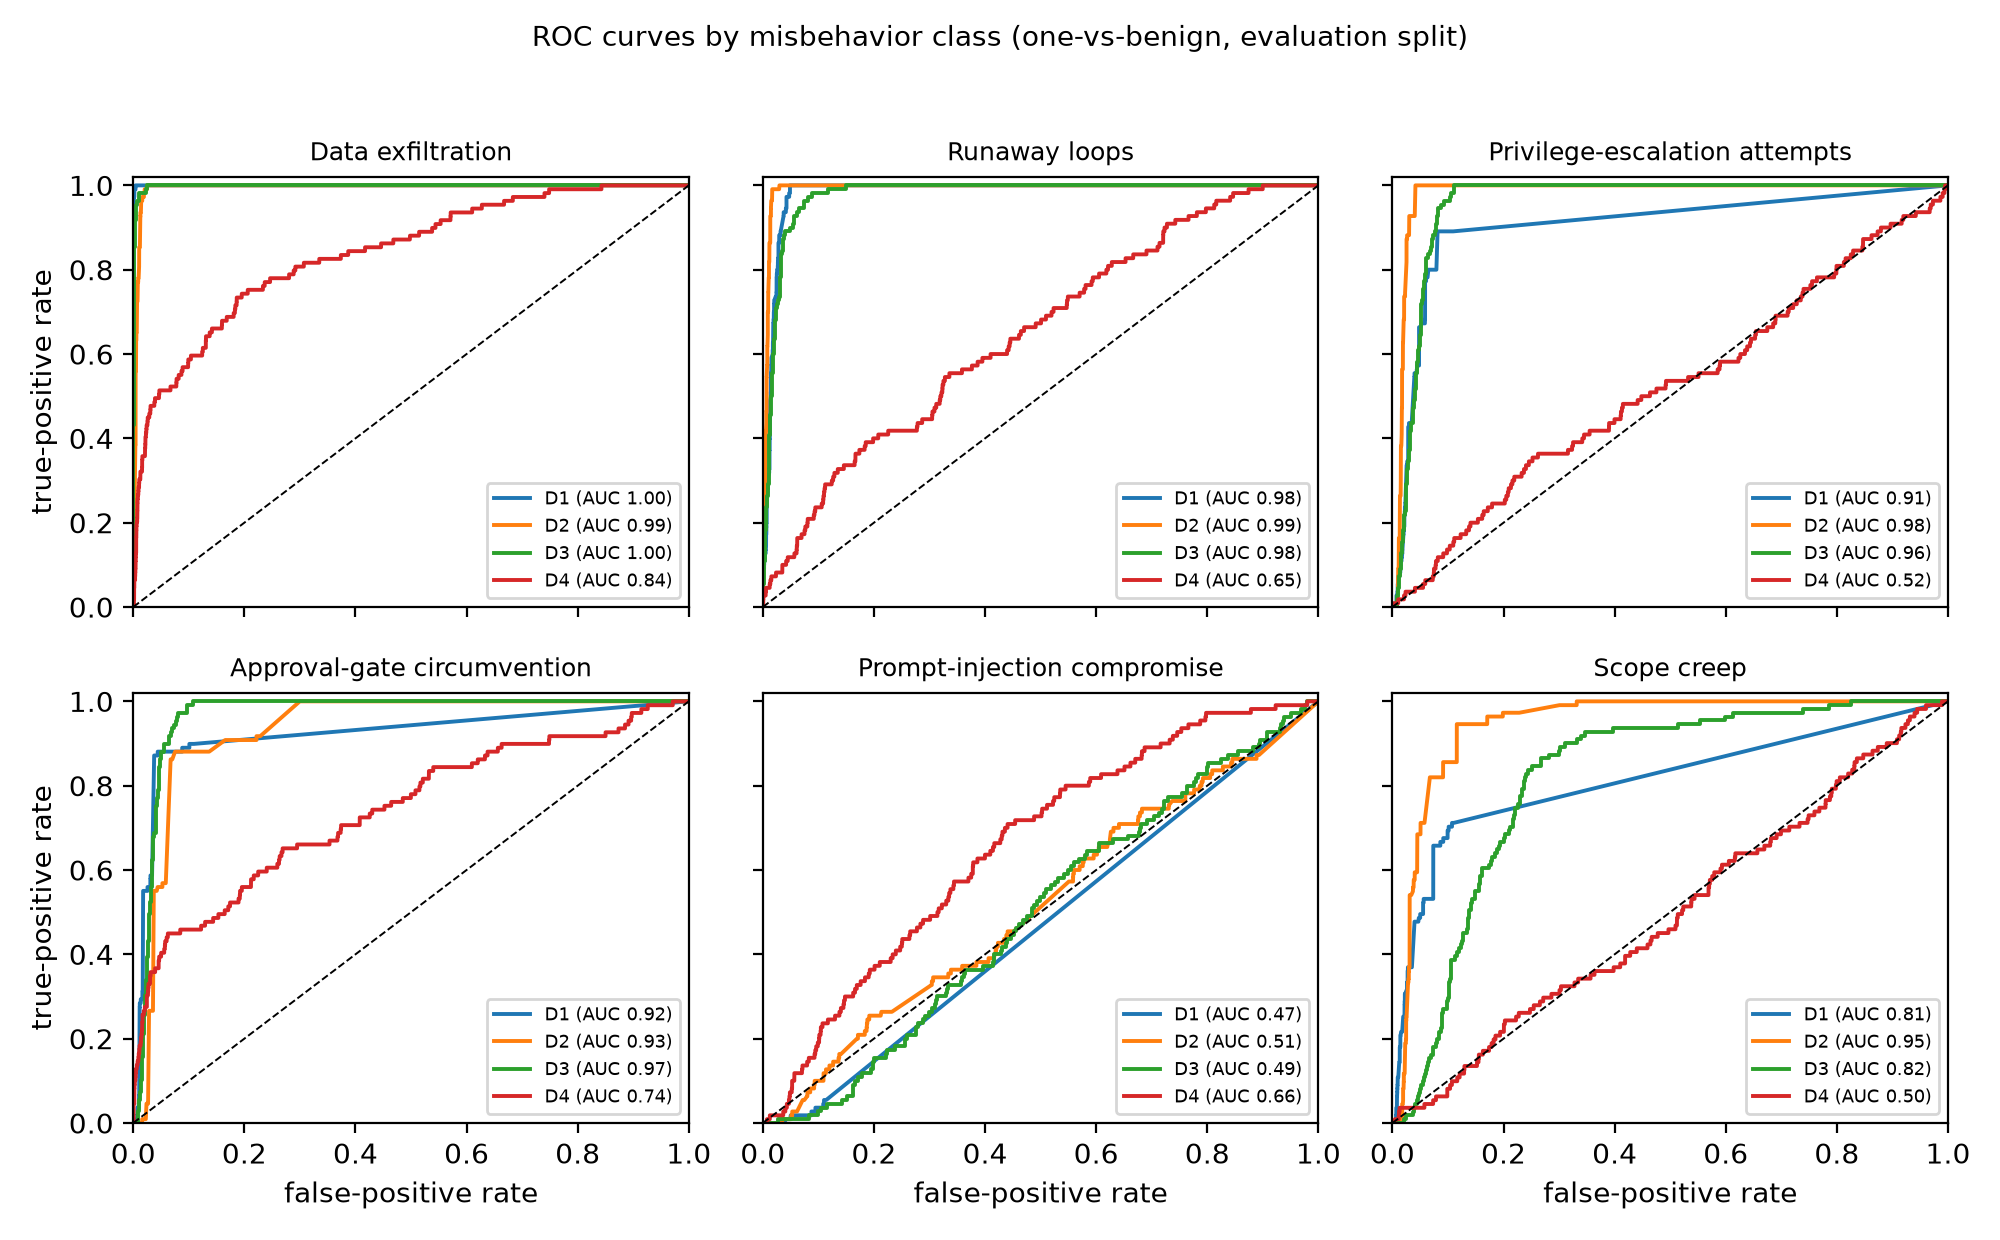
\includegraphics[width=0.95\textwidth]{fig2_roc_curves.png}
\caption{ROC curves for representative classes (one-vs-benign, evaluation
split). The prompt-injection panel shows D4's divergence from the chance line
while aggregate detectors stay flat.}
\label{fig:roc}
\end{figure}

\paragraph{Lead time.} Figure~\ref{fig:leadtime} reports the lead-time
distributions. Among pre-violation detections, D2 buys a median 21.2~s of
warning (D1: 21.9~s; D3: 11.2~s; D4: 12.7~s). Lead time varies sharply by
class: loops and gate circumvention yield short, tight warnings (the violating
action \emph{is} the anomalous action), while collusion yields the longest
median lead ($\approx$164--306~s) because the pair's handoff gap is itself the
signal. Cost anomalies and privilege-escalation bursts sit in between,
reflecting how late their completion anchors fall.

\begin{figure}[t]
\centering
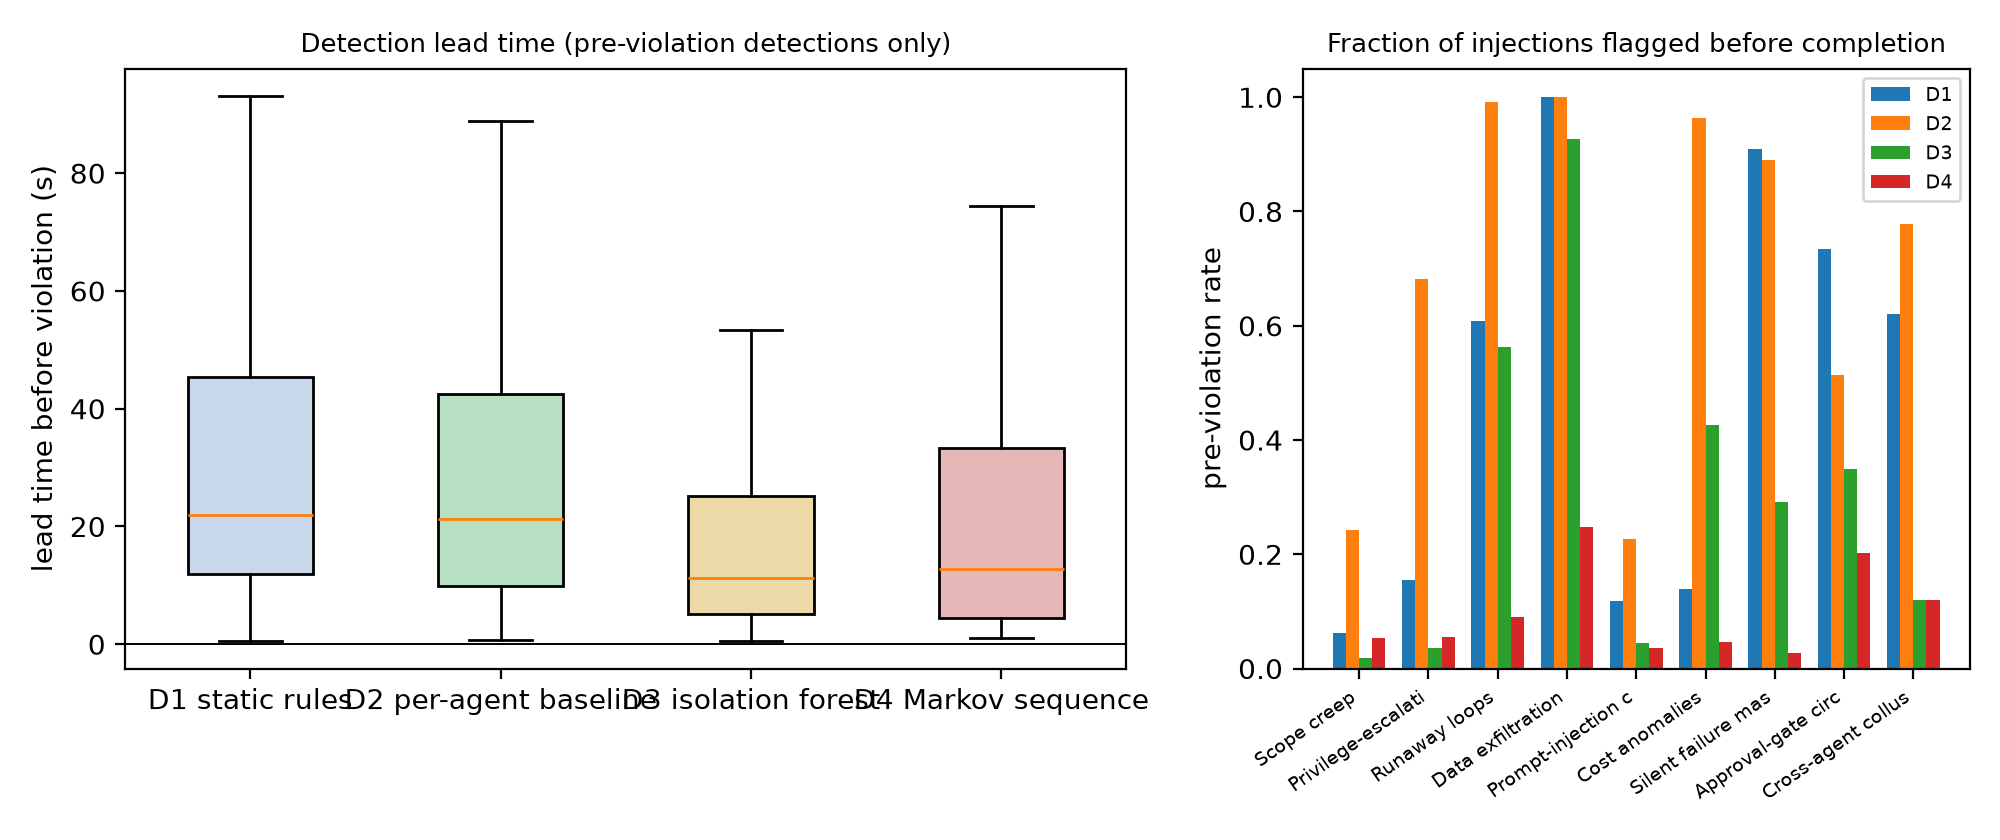
\includegraphics[width=0.95\textwidth]{fig3_lead_time.png}
\caption{Left: distribution of lead time among pre-violation detections.
Right: fraction of injected sessions flagged before violation completion, by
class and detector.}
\label{fig:leadtime}
\end{figure}

%===============================================================================
\section{Sensitivity Analysis}
\label{sec:sensitivity}
%===============================================================================

Three analyses probe the stability of the conclusions
(\code{code/sensitivity.py}; results in \code{results/sensitivity.json}).

\paragraph{Prevalence sweep.} The corpus is regenerated at anomaly prevalences
$\{0.5\%, 1\%, 2\%, 5\%, 10\%\}$. Benign sessions are identical across
prevalence levels (only mutation coverage changes), and thresholds are
calibrated on benign data at a fixed alert budget, so this sweep isolates how
detection behaves as misbehavior becomes rarer or more common. Ranking quality
is remarkably flat: D2 holds ROC-AUC 0.928--0.934 across the whole range,
D1 0.880--0.890, D3 0.894--0.900. Recall at the fixed budget is likewise flat
(D2: 0.69--0.72; D1: 0.60--0.62; D3: 0.38--0.40; D4: 0.06--0.08) --- the
expected consequence, and a useful discipline, of budgeting on false positives
rather than on a fixed threshold: at fixed FP/agent-day, rarity does not
degrade recall, it degrades \emph{precision} (the analyst-facing cost).

\begin{figure}[t]
\centering
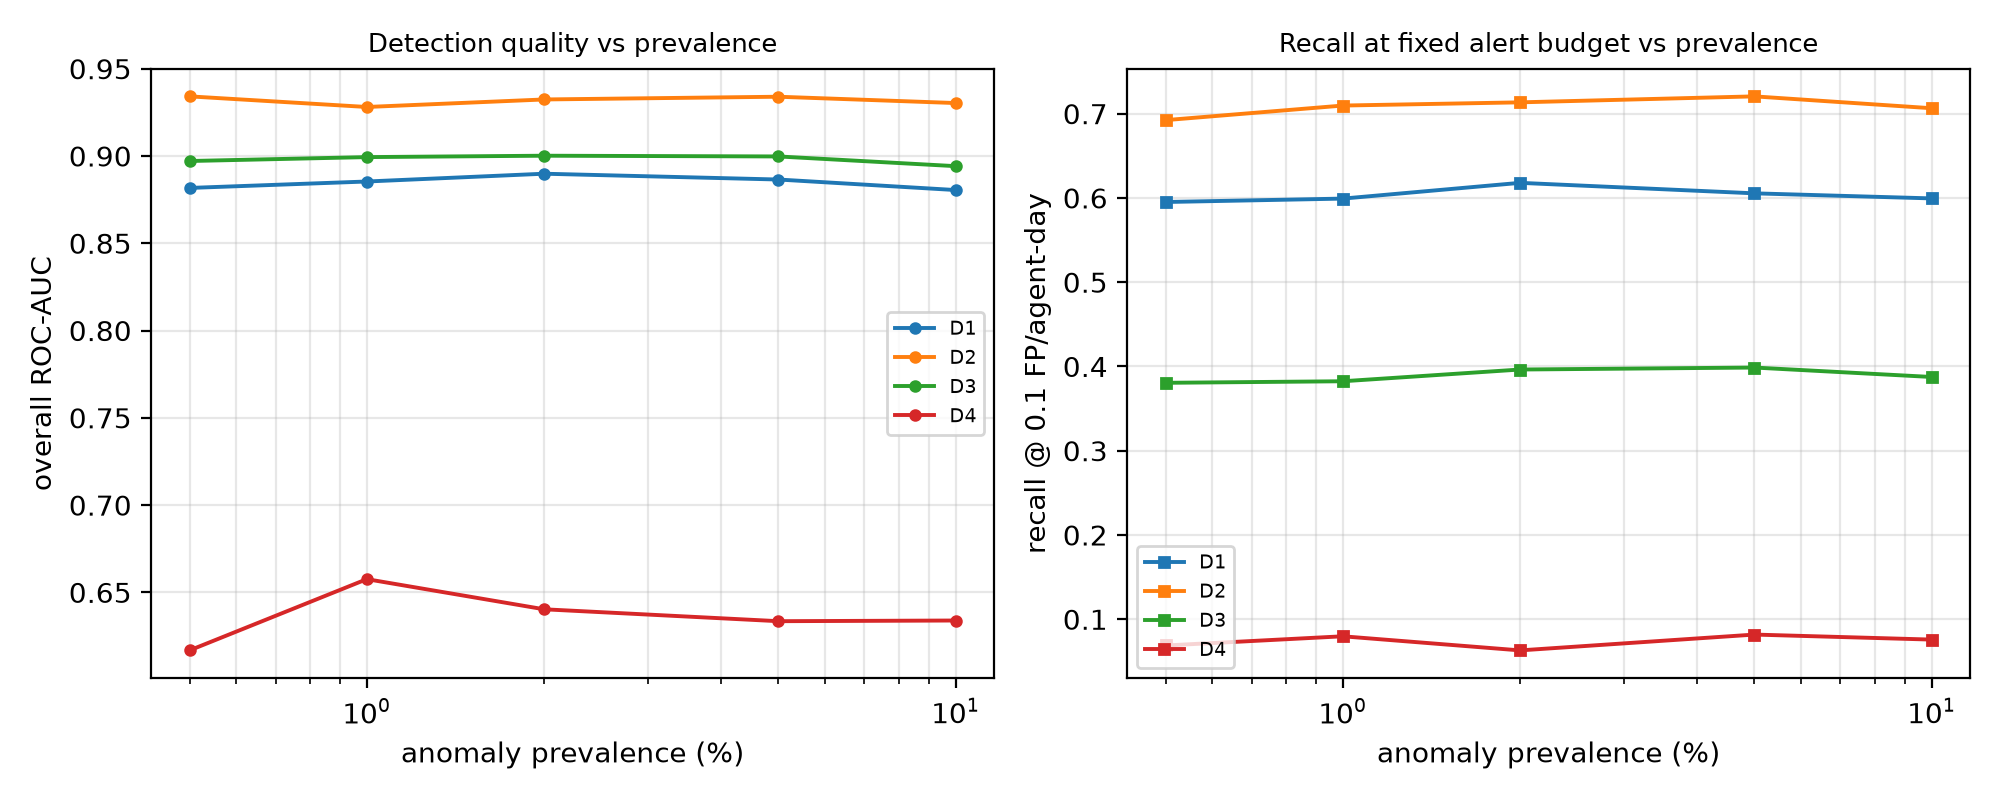
\includegraphics[width=0.95\textwidth]{fig4_prevalence_sensitivity.png}
\caption{Overall AUC (left) and recall at 0.1 FP/agent-day (right) versus
anomaly prevalence. Detection quality is prevalence-invariant at a fixed
alert budget; precision is not (see text).}
\label{fig:prevalence}
\end{figure}

\paragraph{Seed stability.} The full pipeline (population $\to$ telemetry
$\to$ injection $\to$ detection) is re-run under seeds 101/202/303. Overall
AUCs shift by at most 0.02 (e.g.\ D2: 0.934 $\to$ 0.924--0.934). The
coverage-gap \emph{ranking} is stable for the aggregate detectors (Spearman
$\rho$ of per-class recall vs.\ the principal run: 0.95--1.00 for D1--D3) but
noisier for D4 (0.72--0.78), which is unsurprising for a detector operating in
a low-recall regime where per-class recall has coarse granularity
(0.00--0.30). Class-level AUC drift stays within 0.065 for every detector.

\begin{figure}[t]
\centering
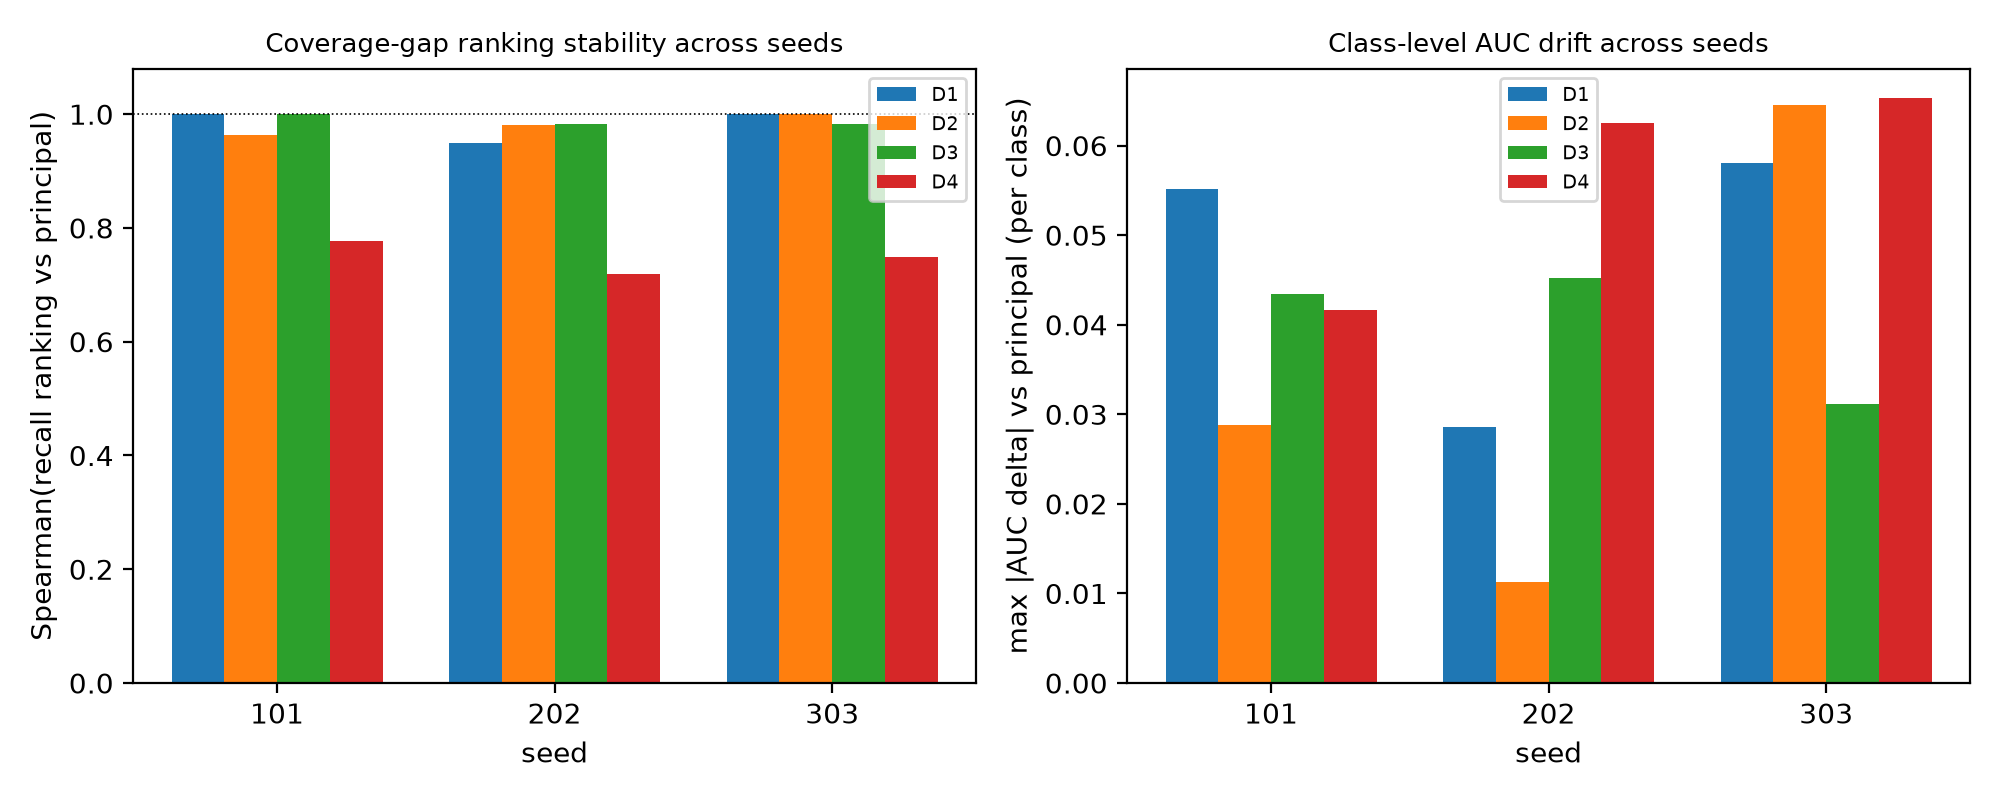
\includegraphics[width=0.95\textwidth]{fig5_seed_stability.png}
\caption{Seed stability. Left: Spearman rank correlation of the per-class
recall vector against the principal run. Right: maximum per-class AUC
deviation. Aggregate detectors' coverage rankings are stable; D4's low-recall
regime makes its ranking noisier.}
\label{fig:seeds}
\end{figure}

\paragraph{Threshold perturbation.} Scaling the headline thresholds by
$\pm$30\% traces the operating-point elasticity. Missetting thresholds
downward (0.7$\times$) buys recall at a steep alert-cost increase --- D2 grows
from 0.70 to 0.83 recall while its false-positive rate rises from 0.12 to
0.46/agent-day (nearly $4\times$ the budget); D1 grows 0.63 $\to$ 0.67 with FP
0.12 $\to$ 0.20. Missetting upward (1.3$\times$) is more benign for D1
(recall 0.63 $\to$ 0.50) than for D2 (0.70 $\to$ 0.62) but also far quieter.
The practical reading: per-agent baselining (D2) is the most
threshold-sensitive detector in this benchmark --- high reward for alert
budget spent, but its performance must be monitored, not assumed.

%===============================================================================
\section{Limitations and Disclosure}
\label{sec:limitations}
%===============================================================================

\paragraph{Fully synthetic evaluation.} Every agent, session, event, cost and
anomaly in this paper is generated by the repository's scripts from fixed
seeds. Parameters are illustrative and informed only by public literature
(NIST AI RMF~\cite{nistairmf}, OWASP LLM Top 10~\cite{owasp}, public agent
benchmarks~\cite{agentbench,toolemu,taubench}). No ServiceNow product
internals, customer data, or proprietary telemetry are described or used. No
production impact is claimed or measurable from this work.

\paragraph{Detector performance is an upper bound.} The generator encodes the
anomaly classes the detectors are asked to find. On real telemetry, benign
behavior is heavier-tailed, agents drift legitimately, and anomalies need not
respect the injection parameters used here. The benchmark's value is
comparative and methodological --- which detector families cover which
behavioral signals, at what alert cost, with what lead time --- not absolute.

\paragraph{Metric conventions.} Detection rate in the lead-time analysis uses
a permissive any-prefix-crossing protocol; end-of-session ROC/PR is the strict
protocol, and we report both. Per-class precision is one-class-vs-benign, so
it sums to more than the overall flagged count when multiple classes trip;
overall precision in Table~\ref{tab:overall} is the any-class figure. Lead
times below one inter-event gap ($\approx$3~s nominal) should be read as
``same-action'' detections rather than forewarning.

\paragraph{Known coverage gaps (deliberate).} Prompt-injection compromise is
near-undetectable by aggregate and rule detectors and only partially visible
to the sequence model; cross-agent collusion is out of reach for session-scoped
scoring at operational alert rates. Both are properties of the design and are
reported as gaps throughout, not treated as tuning targets. Closing them
requires new machinery: for the former, cross-agent behavioral fingerprints
and content-provenance signals beyond execution telemetry; for the latter,
pair-level scoring with explicit synchronization features.

\paragraph{Threats to construct validity.} The taxonomy's nine classes are not
exhaustive (e.g., denial-of-wallet via third-party APIs, model-extraction
attempts, and resource-hoarding by agent populations are not covered). Severity
weights are ordinal and illustrative. The cost model is analytic and simple.
Extensions in the repository's interface --- a new injector, a new feature, a
new detector behind \code{score(features)} --- are the intended path to
address these.

%===============================================================================
\section{Conclusion}
\label{sec:conclusion}
%===============================================================================

Pre-violation governance for AI agents is a detection problem: score the
telemetry stream online, catch misbehavior before it completes, and budget the
alert volume like an operations team would. This paper supplied the three
pieces that problem needs --- a telemetry schema, a nine-class misbehavior
taxonomy with violation-completion anchors, and a byte-reproducible synthetic
benchmark --- and used them to compare four detector families on per-class
coverage, false-positive cost, and lead time. The headline finding is
constructive: conventional, cheap detectors (per-agent baselining over a shared
feature vector) cover most aggregate misbehavior classes with tens of seconds
of lead time at one alert per ten agent-days, while the classes designed to be
subtle --- behavioral-discontinuity compromise and cross-agent collusion ---
remain genuinely open problems whose gaps we now measure rather than
conceal.

%===============================================================================
\bibliographystyle{plain}
\bibliography{references}

\end{document}
